\chapter{Recolección de Datos}\label{chap:recoleccion}

En este capítulo se describirá  los pasos que se llevaron a cabo para obtener los datos de la tesis. Se  desarrollara de manera mas detallada como se obtuvo el dataset y que configuraciones de bandas se usaron para la construcción de las imágenes.


\section{Imágenes Satelitales}

Una imagen satelital se la puede definir como la representación visual de información capturada por un sensor montado en un satélite artificial (Sec:\ref{sub:imagen_satelital}). Estos sensores recogen la información reflejada por la superficie de la tierra que luego es enviada para su posterior procesamiento.

El uso de imágenes satelitales constituye una excelente herramienta para el conocimiento y monitoreo de los territorios y recursos; hoy en día disfrutamos de la oportunidad de aprovechar estas imágenes satelitales para una gran variedad de aplicaciones como: desarrollo y planificación urbana, infraestructura, recursos naturales, investigación, alerta temprana de catástrofes, asuntos militares, entre otras.

Una imagen satelital debe pasar por diferentes niveles de procesamiento dependiendo el tipo de uso que se le quiera dar, en la siguiente sección (Sec:\ref{sub:nivelesdeprocesamiento}) se desarrolla mas en detalle.

\subsection{Niveles de procesamiento}\label{sub:nivelesdeprocesamiento}

En el campo de la teledeteccion (Sec:\ref{sub:teledeteccion}) cuando hablamos de niveles de procesamiento nos referimos a los diversos procesos que son aplicados a una imagen satelital. Dependiendo de la agencia espacial existe una nomenclatura para determinar que niveles de procesamiento fueron aplicados.

En este trabajo se utilizo la nomenclatura propuesta por \ac{nasa}:
\begin{itemize}
	\item \textbf{Nivel 0}: La información científica recogida está a máxima resolución, ordenada temporalmente y con errores de transmisión, artefactos y duplicados eliminados.
 	\item \textbf{Nivel 1a}: La información esta ordenada cronológicamente y datos auxiliares como coeficientes de calibración y parámetros de referencia.
 	\item \textbf{Nivel 1b}: La información del 1a es procesada a unidades de detección, geo-refereciada.
 	\item \textbf{Nivel 2}: Variables geofísicas derivadas por ejemplo productos de concentraciones de hielo, ola de mar, etc.
 	\item \textbf{Nivel 3}: Las variables son mapeadas uniformemente en \textit{grids} espacio-temporales.
 	\item \textbf{Nivel 4}: Resultados de los análisis de los niveles anteriores
\end{itemize}


\section{Datos raw}\label{sec:datosutilizados}

Los datos utilizados para el desarrollo de los experimentos fueron descargadas por medio del catalogo  publicado en el sitio oficial de \ac{conae} \footnote{Fuente: http://catalogos.conae.gov.ar/catalogo/catalogo-de-imagenes.html} de acceso gratuito para el publico. Se debe señalar además que se trabajó con imágenes correspondiente a los años 2017 y 2018 con una ventana de tiempo desde Abril del 2017 a Marzo del 2018; estas imágenes son de naturaleza óptica con un nivel de procesamiento \textbf{1a}, de acuerdo a las nomenclaturas utilizadas en la sección (Sec:\ref{sub:nivelesdeprocesamiento}).

De acuerdo a las característica del proyecto y tomando como fundamentación lo expuesto en la sección (Sec:\ref{sec:fundamentacion}), se utilizaron imágenes que se asemejan a las características del \ac{fs} \ac{conae} detalladas en los requerimientos formales del mismo; estas imágenes fueron adquiridas por el instrumento \ac{viirs} (Sec:\ref{sub:viirs}) a bordo del satélite Suomi-NPP.


Para la realización de diversos experimentos se utilizaron en total 29 combinaciones de bandas \ref{tab:combinacion_banda}, contando con 50 imágenes por cada combinación de bandas que se realizo.


\subsection{Instrumento VIIRS}\label{sub:viirs}
El instrumento \ac{viirs} fue lanzado a bordo del satélite Suomi-NPP el 28 de octubre de 2011. Este instrumento posee 5 canales de alta resolución (I-bands), 16 canales de resolución moderada (M-bands) y un canal de baja luz (Day/Night Band, DNB).  En el siguiente cuadro se detallan las diferentes longitudes de onda y los rangos de onda de las bandas, junto con resolución geométrica apuntando a Nadir (ver tabla: \ref{tab:viirs}).
\begin{table}[H]
\begin{center}
\begin{tabular}{|c|c|c|}
\hline Banda & Rango Espectral (um) & Resolución Nadir \\\hline 
 		M1  & 0.402-0.422   & 0.742 x 0.259 \\ \hline 
		M2  & 0.436-0.454   & 0.742 x 0.259 \\ \hline 
		M3  & 0.478-0.498   & 0.742 x 0.259 \\ \hline 
		M4  & 0.545-0.565   & 0.742 x 0.259 \\ \hline 
		I1  & 0.600-0.680   & 0.371 x 0.387 \\ \hline 
		M5  & 0.662-0.682   & 0.742 x 0.259 \\ \hline 
		M6  & 0.739-0.754   & 0.742 x 0.776 \\ \hline 
		I2  & 0.846-0.885   & 0.371 x 0.387 \\ \hline 
		M7  & 0.846-0.885   & 0.742 x 0.259 \\ \hline 
		M8  & 1.230-1.250   & 0.742 x 0.776 \\ \hline 
		M9  & 1.371-1.386   & 0.742 x 0.776 \\ \hline 
		I3  & 1.580-1.640   & 0.371 x 0.387 \\ \hline 
		M10 & 1.580-1.640   & 0.742 x 0.776 \\ \hline 
		M11 & 2.225-2.275   & 0.742 x 0.776 \\ \hline 
		I4  & 3.550-3.930   & 0.371 x 0.387 \\ \hline 
		M12 & 3.660-3.840   & 0.742 x 0.776 \\ \hline 
		M13 & 3.973-4.128   & 0.742 x 0.259 \\ \hline 
		M14 & 8.400-8.700   & 0.742 x 0.776 \\ \hline 
		M15 & 10.263-11.263 & 0.742 x 0.776 \\ \hline 
		I5  & 10.500-12.400 & 0.371 x 0.387 \\ \hline 
		M16 & 11.538-12.488 & 0.742 x 0.776 \\ \hline 
\end{tabular}
\end{center}\caption{Característica de bandas,\ac{viirs} \label{tab:viirs}}
\end{table}

\subsection{Combinaciones de bandas en canales RGB}\label{sub:comb_de_banda} 
%http://www.gisandbeers.com/combinacion-de-imagenes-satelite-landsat-sentinel-rgb/

Las redes neuronales que vamos a utilizar para la construcción de esta tesis son redes neuronales pre-entrenadas (Sec:\ref{sub:cnn}), estas redes neuronales necesitan como entrada imágenes ópticas con tres canales correspondiente a \textit{RGB} (rojo, verde y azul), los canales RGB se emplean para representar distintos colores a partir de la mezcla de cada uno de estos.

Para construir el dataset de entada a la red se debió convertir los datos \textit{raw} en imágenes tomando como base los canales RGB mencionados. Las combinaciones de bandas en imágenes satelitales nos ayudan a analizar diferentes elementos dentro de la misma imagen, para esto utilizamos diversas combinaciones de bandas en cada canal RGB que que nos muestran diferentes elementos de acuerdo a la banda utilizada. El paso de cada banda por un canal RGB especifico permitirá teñir de colores los elementos que ofrezcan mayor o menor reflexión de longitudes de onda como por ejemplo, la vegetación, focos de incendios, entre otros brindando diversa fuente de información para ser explorada. 

En el siguiente cuadro  \ref{tab:combinacion_banda} se puede ver todas las combinaciones de bandas utilizadas para la construcción del dataset. El conjunto de bandas seleccionadas para los experimentos son las de resolución moderada (M-bands) \ref{tab:viirs} , que posee una resolución espacial a nadir de 750 metros.

\begin{table}[H] \begin{center}
\begin{tabular}{|c|c|}\hline 
Num & Combinación de banda\\ \hline 
1  	& 	M1-M1-M1 	\\ \hline
2  	&   M1-M3-M5	\\  \hline
3  	& 	M1-M5-M3	\\ \hline
4  	&   M3-M1-M5 	\\ \hline
5   & 	M3-M3-M3 	\\ \hline
6   & 	M3-M5-M1 	\\ \hline
7   & 	M5-M1-M3 	\\ \hline
8   & 	M5-M3-M1 	\\ \hline
9   &   M5-M5-M5  	\\ \hline
10  &	M7-M7-M7   	\\ \hline
11  & 	M9-M9-M9   	\\ \hline
12  & 	M11-M7-M9  	\\ \hline
13  & 	M11-M9-M7  	\\ \hline
14  &  	M7-M11-M9  	\\ \hline
15  & 	M7-M9-M11  	\\ \hline
16  & 	M9-M11-M7  	\\ \hline
17  & 	M9-M7-M11  	\\ \hline
18  & 	M11-M11-M11	\\ \hline
19  & 	M11-M13-M15 \\ \hline
20  & 	M11-M15-M13 \\ \hline
21  & 	M13-M11-M15 \\ \hline
22  & 	M13-M13-M13	\\ \hline
23  & 	M13-M15-M11 \\ \hline
24  & 	M15-M11-M13	\\ \hline
25  & 	M15-M13-M11	\\ \hline
26  & 	M15-M15-M15 \\ \hline
27  & 	M5-M4-M3 	\\ \hline
28  & 	M10-M7-M5 	\\ \hline   
29  & 	M11-M12.M13	\\ \hline        	
\end{tabular}
\end{center}\caption{Combinaciones de bandas utilizadas \label{tab:combinacion_banda}}
\end{table}

En la siguiente figura \ref{Fig: bandas543} podemos visualizar unas de las imágenes que se utilizo; en este caso corresponde  a las combinaciones de bandas M5, M4, M3 conocidas como color verdadero, \textit{true color} su nombre en ingles .

\begin{figure}[H]
 \centering
  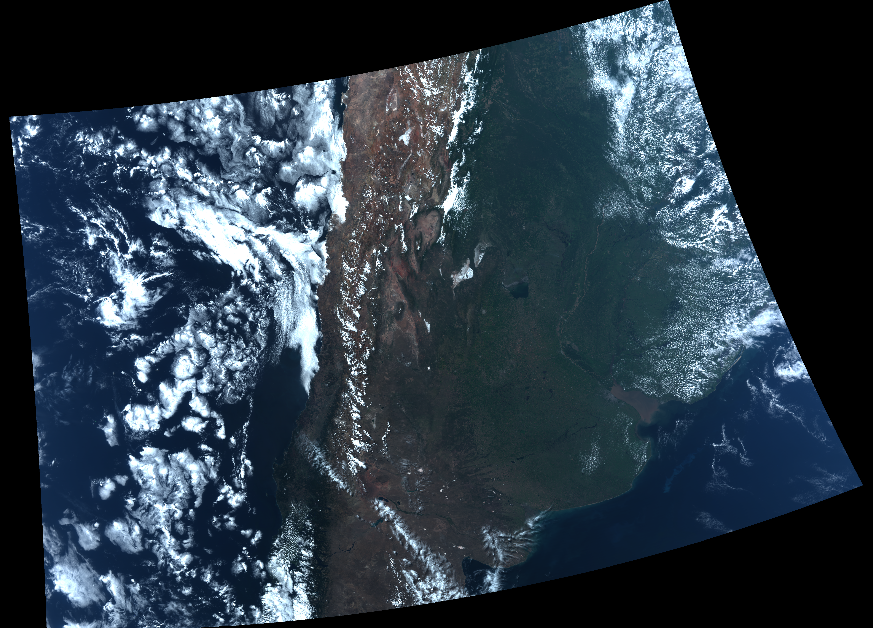
\includegraphics[height=10cm,keepaspectratio=true,clip=true]{imagenes/recoleccion/img-543.png}
  \caption{Combinación de bandas M5, M4 y M3}
	\label{Fig: bandas543}
\end{figure}

